\documentclass[a4paper,12pt]{article}
\usepackage[utf8]{inputenc}
\usepackage[spanish]{babel}
%\usepackage{graphicx}
\usepackage[pdftex]{graphicx} 
\graphicspath{ {images/} }
\DeclareGraphicsExtensions{.jpeg,.png,.jpg}  
\usepackage{tikz}

% Taken from Lena Herrmann at 
% http://lenaherrmann.net/2010/05/20/javascript-syntax-highlighting-in-the-latex-listings-package
\usepackage{listings}
\usepackage{color}
\definecolor{lightgray}{rgb}{.9,.9,.9}
\definecolor{darkgray}{rgb}{.4,.4,.4}
\definecolor{purple}{rgb}{0.65, 0.12, 0.82}

\lstdefinelanguage{JavaScript}{
  keywords={typeof, new, true, false, catch, function, return, null, catch, switch, var, if, in, while, do, else, case, break},
  keywordstyle=\color{blue}\bfseries,
  ndkeywords={class, export, boolean, throw, implements, import, this},
  ndkeywordstyle=\color{darkgray}\bfseries,
  identifierstyle=\color{black},
  sensitive=false,
  comment=[l]{//},
  morecomment=[s]{/*}{*/},
  commentstyle=\color{purple}\ttfamily,
  stringstyle=\color{red}\ttfamily,
  morestring=[b]',
  morestring=[b]"
}

\lstset{
   language=JavaScript,
   backgroundcolor=\color{lightgray},
   extendedchars=true,
   basicstyle=\footnotesize\ttfamily,
   showstringspaces=false,
   showspaces=false,
   numbers=left,
   numberstyle=\footnotesize,
   numbersep=9pt,
   tabsize=2,
   breaklines=false,
   showtabs=false,
   captionpos=b,
%   aboveskip=20pt,
   belowskip=25pt
}


%\usetikzlibrary{snakes}
\usetikzlibrary{decorations}

\title{Estudio del Comportamiento del Ganado en Sistemas Distribuidos con Caracteres Autónomos}
\author{María Losada \and Estefanía Valenzuela \and Laura Zorrilla}
\date{09/JUNIO/2014}

\begin{document}
\newcommand{\lluvia}{\textbf{\textit{lluviaProject}}}

\section*{}
\label{chap:prologo}

Este proyecto no podría haberse completado sin la colaboración de José Luis Álvarez y José María González, a los que desde aquí queremos 
agradecer su ayuda.

\tableofcontents

\section{Introducción}
\label{sec:introduccion}

\subsection{¿De qué trata el juego?}
\label{subsubsection:intro_juego}

En este proyecto hemos querido plasmar el comportamiento de un rebaño de ovejas ante el movimiento del pastor y el entorno que las rodea. 
Nuestra finalidad es hacer que la simulación del comportamiento de estos animales en el videojuego sea lo más cercana posible a los hábitos 
y reacciones de aquellos. \\

Tan importante es el comportamiento del ganado como del pastor. Es por eso que, además, se realizaron investigaciones sobre las técnicas y 
las estrategias de pastoreo. El estudio de estos comportamientos y las investigaciones realizadas al respecto permiten determinar que al 
ganado se le puede agrupar, induciendo su comportamiento natural de permanecer unidos. Para ello hay varias técnicas:

\begin{itemize}
 \item Técnica del limpiaparabrisas: El pastor debe moverse en zigzag de un lado a otro de la manada para mantener la línea recta de avance. Figura 1.1.1

 \item Moverlos por el apretadero : Los animales necesitan tener el suficiente espacio para moverse adecuadamente.

 \item El pastor debe de tener movimientos lentos y no debe dar vueltas alrededor de los animales.

 \item Zona de fuga: La zona de fuga de un animal es su zona de seguridad. Los operarios deben mantenerse en el límite de esta zona.Figura 1.1.2

 \item Movimiento del pastor para que el ganado siga su camino en una manga con laterales: Para obligar al animal a desplazarse hacia adelante, el pastor debe estar por detrás del punto de equilibrio a la altura de los cuartos delanteros.

 \item Sacar al ganado del corral con un solo controlador: Los movimientos del pastor deben de ser perpendiculares a los del ganado, moviéndose hacia atrás y hacia delante sobre la barra transversal de una gigante T.

 \item Sacar al ganado del corral con dos controladores:  Cada pastor se moverá hacia detrás y hacia delante en la línea transversal imaginaria que traza una T.
\end{itemize}

\subsubsection{Comportamientos del Ganado Ovino}
\label{subsubsection:comportamientos}

Los animales siguen al líder. Si éstos se despistan y se amontonan, el pastor debe concentrarse en mover a los líderes en lugar de empujar 
al grupo de animales de la parte trasera. Al mover al ganado en un espacio abierto, los animales se mueven en una forma tranquila y ordenada.\\

Para acelerar el paso de los animales, los pastores penetran la zona de fuga colectiva y se retiran. El campo de visual de las ovejas puede 
ser de 191 hasta 309 grados, dependiendo de su cantidad de lana.\\

Los animales de pastoreo tienen un sistema visual que proporciona una excelente visión de lejos, pero los músculos de los ojos relativamente 
débiles les inhiben de la capacidad de centrarse rápidamente en los objetos cercanos.\\

La implementación de estos comportamientos en este proyecto implica un lenguaje de programación capaz de reproducir lo explicado anteriormente.
De los lenguajes disponibles para realizar aplicaciones, \lluvia{} era el único que disponía de caracteres personales autónomos, los cuales permiten modelar su 
comportamiento para adaptarse al de un rebaño de ovejas.



%\tikzstyle{level 1}=[sibling angle=120]
%\tikzstyle{level 2}=[sibling angle=60]
%\tikzstyle{level 3}=[sibling angle=30]
%\tikzstyle{every node}=[fill]
%\tikzstyle{edge from parent}=[snake=expanding waves,segment length=1mm,segment angle=10,draw]

%\tikz [grow cyclic,shape=circle,very thick,level distance=13mm,cap=round]
%  \node {} child [color=\A] foreach \A in {red,green,blue}
%     { node {} child [color=\A!50!\B] foreach \B in {red,green,blue}
%        { node {} child [color=\A!50!\B!50!\C] foreach \C in {black,gray,white}
%           { node {} }
%        }
%     };

\section{Por qué Lluvia Project}
\label{section:por_que}

\subsection{¿Qué es lluviaProject?}
\label{subsection:que_es}

Es una API Open Source de Javascript que incorpora parte de las funciones nativas de Ruby. Soporta multihilos a pequeña escala y provee un 
sistema de mensajes. Las aplicaciones deben crearse dentro del directorio Vendor. \\

La aplicación debe de contar con un archivo generalmente llamado Dependencies.js, donde deben incluirse el nombre de los ficheros de los que 
depende la aplicación. Si existe una función main esta se llama automáticamente después de cargarse \lluvia.\\

Ver ejemplo en figura 2.1.1


\subsection{Ventajas}
\label{subsection:ventajas}


Una de las funcionalidades que ofrece \lluvia{} es el objeto Boid. A este objeto se le puede configurar tanto el comportamiento como las 
características físicas de aquello que se quiere representar.\\

En la parte física, se puede modelar tanto el peso, la visión, la velocidad, la posición, la aceleración, capacidad de frenada, la capacidad 
de giro, etc. Y por otra parte, se pueden modelar comportamientos de huida, de persecución, de cohesión, de alineamiento, de separación e 
incluso comportamientos hechos a medida. Esta característica de \lluvia{} permite representar los comportamientos de animales, objetos 
o partículas, entre otros.\\

Esto, junto con el hecho de que añade librerías y funciones que hacen que la escritura de código en Javascript sea más cómodo, nos hizo 
decidirnos por \lluvia{}.\\

\section{Parte gráfica}
\label{chap:grafica}

\subsection{Front-end (HTML/CSS)}
\label{sec:front_end}

Esta aplicación multiplataforma ha sido diseñada para ser lanzada desde cualquier navegador. La página tendrá como dimensiones 1200 x 800. 
Está al iniciarse muestra dos controles, botón Play y botón Menú. Ver figura \ref{fig:figura313} en página \pageref{fig:figura313}.\\

El botón Play inicia el juego mostrando una pantalla en la que aparecen un cerdito y un rebaño de ovejas. El cerdito hace la labor de pastor, 
teniendo que meter un número determinado de ovejas en el corral para poder pasar al siguiente nivel. 
En la esquina superior izquierda se encuentra el cronómetro, inicializado en dos minutos y realiza la cuenta atrás hasta llegar a cero.
A la derecha de éste se encuentra un contador, que irá aumentando según el número de ovejas que vayan entrando en el redil.
En la esquina superior izquierda está situado el menú de la aplicación que está compuesto por las siguientes opciones:

\begin{itemize}
 \item Instructions: Donde se explica el funcionamiento del juego.
 \item Restart level: Permite reiniciar el nivel.
 \item Levels: Muestra los niveles del juego que se irán desbloqueando según se vayan superando.
\end{itemize}

A su izquierda se sitúa el botón para activar y desactivar la música de fondo. La imagen de éste variará dependiendo de si la música 
está en reproducción o en silencio.\\

El diseño de la página principal tuvo varios procesos. La evolución que siguió está representada en las imágenes: figura \ref{fig:figura311}, figura \ref{fig:figura312} y 
figura \ref{fig:figura313}.


\subsection{Canvas}
\label{sec:canvas}

El elemento Canvas  de HTML5 es un contenedor gráfico que  proporciona a los scripts  un mapa de bits  que funciona como lienzo.
Lo primero que se debe de hacer es referenciar el elemento Canvas dándole unas dimensiones, 851 x 424 (ancho y largo) y adquirir su contexto.
En este caso hemos utilizado un contexto bidimensional (2D).\\

Dentro del archivo HTML es necesario incluir en la 
etiqueta body llamar a la función Bring\_LLuvia().\\

El lenguaje de programación Javascript contiene una serie de funciones propias que nos permiten  a través de coordenadas dibujar en el Canvas.
Estas son algunas de ellas.

\begin{itemize}
 \item beginPath():  Con esta función se da por comenzado el trazo.
 \item moveTo(x, y): Coloca el cursor en el punto de inicio y a partir de ahí, se va creando la forma de la figura a través de las distintas 
 funciones.
 \item lineTo(x, y): Traza líneas rectas desde una coordenada a otra.
 \item fill(): Dibuja una forma cerrada con el color de relleno actual. Si la forma no está cerrada, la propia función crea una línea recta 
 desde el punto de inicio  al punto final para cerrarla.
 \item arc(x, y, radio, ángulo inicial, ángulo final, sentido de giro):  Se utiliza para dibujar circunferencias y arcos.
 \begin{enumerate}
 \item x, y: Son las coordenadas del centro de la circunferencia.
 \item Radio: Radio de dicha circunferencia.
 \item Ángulo inicial y ángulo final: Marca la amplitud del arco desde el ángulo inicial al ángulo final en el sentido de las agujas del reloj. Los ángulos se miden en radianes. 
 La equivalencia con los grados nos la da esta expresión:\\
 radianes = (Math.PI/180)*grados
 \item El sentido de giro tiene el valor lógico cierto, el arco irá en sentido contrario a las agujas del reloj. Este último parámetro es 
 opcional y por defecto su valor es falso.
 \end{enumerate}
 \item closePath(): Crea una línea recta desde el último punto al punto inicial. Da por finalizada la figura.
\end{itemize}

Gracias a HTML5, CSS3 y Javascript, hemos podido realizar tanto el fondo del juego, como las figuras que representan a los personajes.
Al igual que en la pantalla principal, los elementos del Canvas han sufrido varios procesos, a medida que se ha ido mejorando la técnica de creación, éstos han ido cambiando.
Se puede ver un ejemplo en las figuras \ref{fig:figura321} (página \pageref{fig:figura321}), \ref{fig:figura322} (página \pageref{fig:figura322}), 
\ref{fig:figura323} (página \pageref{fig:figura323}), \ref{fig:figura324} (página \pageref{fig:figura324}) y \ref{fig:figura325} (página \pageref{fig:figura325}).

\section{Clases}
\label{sec:clases}

\subsection{Estructura de una clase}
\label{subsection:estructura}

\lluvia, al igual que otros lenguajes orientados a objetos, está organizado en clases.\\

Para crear una clase es necesario definir una función constructora. 
\begin{verbatim}
 var myClass = function() {;} 
\end{verbatim}

Ésta puede contener atributos y métodos públicos accesible sólo desde la clase, que no se pueden heredar y que se definen como:
\begin{verbatim}
myClass.attribute = VALUE
myClass.method = function(){;}
\end{verbatim}

También se pueden definir atributos y métodos heredables por aquellos objetos que derivan de la clase. 
Para esto, es necesario añadir prototype entre el nombre de la clase y el nombre del atributo o método. 
\begin{verbatim}
myClass.prototype.attribute = VALUE
myClass.prototype.method = function(){;}
\end{verbatim}

Las variables y métodos privados se definen dentro de la función como
\begin{verbatim}
var attribute = VALUE
\end{verbatim}

Una clase puede devolver una variable o un objeto complejo, llamado cierre, con capacidad para acceder a más de un atributo. 
De esta manera, una clase puede ser, a su vez, una factoría de objetos.
\begin{verbatim}
var derived_class = new myClass()
\end{verbatim}

Estas clases pueden aceptar parámetros o no y new es opcional.\\

Aunque \lluvia{} no define nada al respecto, los cierres se suelen usar a través de la función yield, la cual busca entre los parámetros 
un objeto función y lo ejecuta.\\

Las clases aceptan un objeto de configuración, el cual permite modificar la propia clase en caso necesario. Al igual que en javascript, 
no es necesario definir el tipo de las variables. Ver ejemplo en código \ref{lst:code411} (página \pageref{lst:code411})\\

\lluvia{} permite definir una función dentro de la propia clase. Ver ejemplo en código \ref{lst:code412} (página \pageref{lst:code412})\\

La palabra reservada this, dentro del ámbito de new, hace referencia al objeto que se está creando, mientras que fuera de él hace 
referencia al objeto que se está ejecutando.\\

\textbf{Object\#method\_missing:} \\
Cuando una función no existente es llamada, se levanta una excepción y se llama al método method\_missing()



\subsubsection{Cadena Prototípica}
\label{subsubsection:prototipos}

Las clases siguen las convenciones de las cadenas prototípicas de Javascript. Esto quiere decir que si el atributo no está presente en el 
objeto, entonces se mira en el constructor de la clase padre. Si ésta deriva a su vez de otra, entonces se busca en el constructor del 
padre de la segunda. Ver figura figura \ref{fig:figura413} (página \pageref{figura:figura413})\\

Aquellas funciones definidas sin la palabra reservada prototype no son accesible por ninguna instancia de la clase. Tanto éstas como aquellas 
funciones que no que no acceden a los atributos de clase se consideran estáticas.\\

Es posible definir métodos singleton, que se crean en el constructor de la clase y que no pertenecen a la clase padre. Dentro de estos 
métodos, this pierde su significado y es necesario que esté recogido en una variable local para poder acceder a él.\\



\subsection{Clase Boid}
\label{subsection:boid}

\subsubsection{Introducción}
\label{subsubsection:boid_general}

Un Boid se define como un carácter personal autónomo que recibe un objeto de configuración y un bloque. Al crear una nueva instancia, se 
le puede pasar como parámetro un objeto de configuración y/o un bloque de código. Si se le pasa un objeto de configuración, es necesario 
definir todos los parámetros a incluir en el constructor del nuevo Boid. Si se le pasa un bloque, se pueden definir sólo aquellos parámetros 
que vayan a cambiar con respecto a la clase padre.\\

La configuración por defecto incluye un objeto geo\_data, el cual contiene los atributos de posición, velocidad y aceleración, color del 
boid, un cerebro, velocidad máxima, masa, el objeto vision, con radio y ángulo, y el objeto límites dinámicos, que incluye capacidad de 
empuje, de giro y de frenada. Ejemplo de configuración por defecto. Código \ref{lst:code4211} (página \pageref{lst:code4211})\\

Es posible modificar su posición, velocidad o aceleración en tiempo real según sea necesario. También se le puede asignar un comportamiento 
de los que ya existen o crear nuevos que cubran necesidades más específicas.\\

Cada Boid tiene acceso directo a la descripción geométrica de la escena, pero los comportamientos de manada requieren que éste reaccione 
sólo a aquellos boids que se encuentren dentro de un área específica alrededor de él. Este área se define por una distancia, medida desde 
el centro del Boid, y un ángulo, medido en la dirección de avance del Boid. Aquellos Boids que se encuentran fuera de este área son ignorados. 
Ver figura \ref{fig:figura4212} (página \pageref{fig:figura4212})\\


Métodos:
\begin{itemize}
 \item position():
Obtiene o define la posición del Boid

  \item velocity():
Obtiene o define la velocidad del Boid

  \item acceleration():
Obtiene o define la aceleración del Boid

  \item start():
Guarda la hora que marca el procesador.

  \item delta\_at():
Tiempo que ha pasado desde la última vez que la variable 'last time' fue actualizada

  \item update\_physics():
Calcula la nueva posición, velocidad y aceleración en función del tiempo que ha pasado.

  \item run():
Actualiza el tiempo en las variables del Boid.

  \item first\_draw():
Pinta el Boid y lo guarda como imagen, lo que ahorra tiempo de cálculo.

  \item draw():
Pinta un Boid en un mundo definido por un contexto.

  \item heading():
Alinea el vector normal con el último vector de dirección del Boid.

  \item locale():
Expresa las coordenadas locales del sistema en coordenadas globales.

  \item globale():
Expresa las coordenadas globales del sistema en coordenadas locales.

  \item localize():
Cambia las coordenadas globales del sistema en coordenadas del Boid.

  \item globalize():
Cambia las coordenadas locales del sistema en coordenadas del mundo.

  \item visible\_objects():  
Pregunta al mundo si existe un objeto visible dentro de las habilidades de visión y las coordenadas de velocidad, aceleración y posición.
del Boid.

  \item requested\_acceleration(): Devuelve al mundo la aceleración requerida (lo que el cerebro desea y lo que el cuerpo permite).

  \item clip():
Ajusta la aceleración en función de los límites dinámicos del Boid.

  \item set\_target():
Define un target.

  \item  target\_data():
Devuelve la información del target.
\end{itemize}



\subsubsection{Clase Brain}
\label{subsubsection:brain}

Es la clase que crea un cerebro para el Boid. En ella, se guardan los comportamientos disponibles para ser activados. Todos estos 
comportamientos conocidos se guardan en la variable \textit{catalog}. El cerebro, además, se encarga de discriminar entre aquellos que pueden ser activados por 
un Boid concreto y los que no.\\

Guarda las aceleraciones que posee el Boid para cada uno de sus comportamientos activos. De esta manera, se puede calcular la aceleración que 
el Boid necesita para cambiar su posición en función del objetivo.\\


Métodos:
\begin{itemize}
\item can\$U():
Comprueba si el Boid puede activar un comportamiento específico.

\item can\_be\_in\$U():
Comprueba si un comportamiento puede ser activado para un Boid.

\item activate():
Activa un comportamiento determinado en un Boid.

\item deactivate():
Desactiva un comportamiento determinado en un Boid.

\item is\_in\$U():
Comprueba si un comportamiento está en la lista de aquellos aceptados por el Boid.

\item get\_behavior():
Obtiene el comportamiento pasado como parámetro

\item \$see\_accelerations():
Muestra las aceleraciones guardadas por el método desired\_accelerations()

\item desired\_accelerations():
Guarda las aceleraciones de un determinado Boid para todos sus objetivos

\item desired\_acceleration():
Calcula la aceleración que el Boid necesita para cambiar su posición.
\end{itemize}



\subsubsection{Clase Sheep}
\label{subsubsection:sheep}

La clase oveja deriva de la clase Boid, por lo que hereda la mayoría de su funcionalidad. La diferencia fundamental con la clase padre es 
la creación de nuevas funciones y la redefinición de métodos ya existentes.\\

Métodos:
\begin{itemize}
\item sheep\_limits(): Define los límites entre los que los Boids oveja se pueden mover. Esta función es necesaria para que éstos no se 
salgan de los límites impuestos por el canvas. Ver código \ref{lst:code4231} (página \pageref{lst:code4231})

\item  update\_physics(): Calcula la nueva posición, velocidad y aceleración en función del tiempo que ha pasado. Esta función ha sido 
necesaria redefinirla para poder llamar a la función sheep\_limits(). Además, se comprueba si el Boid oveja ha entrado en el corral y, en 
caso afirmativo, se suma un punto al contador. Ver código \ref{lst:code4232} (página \pageref{lst:code4232})

\item  first\_draw():  Pinta el Boid y lo guarda como imagen, lo que ahorra tiempo de cálculo. Se redefine para evitar que los Boids se 
pinten como círculos, ya que en el constructor se determina una imagen para representar a las ovejas. Ver código \ref{lst:code4233} (página \pageref{lst:code4233})

\item  draw(): Pinta un Boid en un mundo definido por un contexto. La diferencia con el método original es que ya no se pintan líneas en 
el canvas. Si la velocidad es mayor que cero, se carga la imagen de la oveja mirando hacia la izquierda y si no, hacia la derecha. 
Ver código \ref{lst:code4234} (página \pageref{lst:code4234}).

\end{itemize}



\subsubsection{Clase Pig}
\label{subsubsection:pig}

La característica principal de esta clase es su capacidad para responder a las coordenadas del ratón cuando el usuario dispara el evento 
onClick(). Éstas son capturadas por el objeto MouseCoordinates, el cual deriva de la clase Gate. A través de su método do\_onclick(), 
transforma las coordenadas globales de la pantalla en locales del canvas y las guarda en sendas variables de clase. Estas variables se 
pasan a la clase World como parámetros de su función move\_shepherd() y se usan para definir el objetivo del Boid, el cual tiene programado un 
comportamiento de persecución. Ver figura \ref{fig:lock} (página \pageref{fig:lock})\\

Métodos:\\

Esta clase cuenta con dos métodos, modificados de la clase original. Al igual que en la clase Sheep, ha sido necesario redefinir 
first\_draw() y draw() para poder cargar la imagen del cerdito en lugar de pintar el círculo que se crea por defecto para representar el 
Boid.



\subsection{Clase Behavior}
\label{subsection:behavior_section}

\subsubsection{Introducción}
\label{subsubsection:behavior}

La clase Behavior permite modelar el comportamiento de los Boid. Esto se consigue modificando el vector de aceleración que cada uno de los 
Boids posee como parte de su estructura interna. Un comportamiento se puede definir como un objeto que devuelve una aceleración deseada en 
un momento concreto.\\

Al ser una clase abstracta, no permite crear instancias, de manera que para crear un comportamiento nuevo es necesario generar una clase 
nueva que derive de ésta.

\begin{verbatim}
Modo incorrecto de crear un comportamiento:

var a = new Behavior()

Modo correcto:

NewBehavior.prototype = new Behavior\\
\end{verbatim}

Estos comportamientos puede tener pre y post modificadores. Los primeros modifican la aceleración antes de devolverla y los segundos,
después. Un ejemplo de premodificador es forsee, que se encarga de calcular dónde estará el objetivo en la próxima medida de tiempo. Este 
premodificador unido al comportamiento de búsqueda seek hacen que varíe la aceleración para modificar la trayectoria y perseguir al objetivo. 
Un ejemplo de premodificador sería arrival, el cual va disminuyendo la aceleración a medida que se acerca al objetivo.\\

Los comportamientos disponibles para los Boids en este momento son seek (búsqueda), flee (huida), wander (paseo), containment (contención 
en el espacio), alignment (alineamiento con otro Boids), cohesion (acercamiento a otros Boids), separation (separación de otros Boids) y 
obstacle avoidance (sorteo de obstáculos).\\

Métodos:
\begin{itemize}
\item decompose\_name():
Dada una cadena de caracteres que representa el nombre del comportamiento y sus modificadores, devuelve un array con la lista de pre
modificadores, el nombre del comportamiento y una lista con los post modificadores.

\item catalog():
Lista todos los comportamientos y modificadores conocidos.

\item new():
Crea un nuevo comportamiento.

\item type\_of():
Devuelve la clase asociada con el nombre del comportamiento.

\item is\_a\$U():
Comprueba si el nombre pasado como parámetro se corresponde con uno de los comportamientos existentes.

\item desired\_acceleration():
Devuelve un vector con la aceleración deseada de ese comportamiento.

\item is\_premodified\_by\$U():
Devuelve true si el nombre del modificador está en la lista de pre modificadores

\item is\_postmodified\_by\$U():
Devuelve true si el nombre del modificador está en la lista de post modificadores.

\item is\_modified\_by\$U():
Devuelve true si el nombre del modificador está tanto en la lista de pre como de post modificadores.

\item get\_modifiers\_for():
Devuelve una lista de pre o post modificadores.

\item all\_modifiers():
Devuelve una lista de todos los modificadores.

\item activate\_modifier():
Activa un modificador determinado.

\item get\_modifier():
Busca un modificador determinado y devuelve null si no lo encuentra.

\item deactivate\_modifier():
Desactiva un modificador determinado.
\end{itemize}


\subsubsection{Clase Sheep Behavior}
\label{subsubsection:sheep_behavior}

Es la clase encargada de generar el comportamiento de las ovejas. Deriva de la clase Behavior. Cuando el cerdito oveja entra dentro del 
radio de visión de la oveja, esto despierta en ella un comportamiento de huida. Es decir, aumenta su aceleración hasta su límite para 
disminuir ésta gradualmente a medida que se va alejando del Boid cerdito.\\

Éste es el primero de los cinco comportamientos que se quieren implementar (véase cuadro \ref{table:nonlin} en la página \pageref{table:nonlin}). Los otros cuatro quedan para una fase 
posterior de desarrollo.\\

Métodos:
\begin{itemize}
\item set\_target():
Define el objetivo del Boid, que debe ser otro Boid y el cual se pasa como parámetro.

\item target\_data():
Define la información sobre la posición del Boid objetivo.

\item get\_target():
Devuelve la posición del objetivo.

\item target\_at():
Da la distancia entre el Boid y su objetivo.

\item desired\_velocity():
Devuelve la velocidad deseada del Boid. Ver código \ref{lst:code4322} (página \pageref{lst:code4322})

\item desired\_acceleration():
Devuelve la aceleración deseada del Boid.
\end{itemize}


\subsubsection{Clase Alignment Behavior}
\label{subsubsection:alignment_behavior}

Al comportamiento básico de la oveja se le añadió el comportamiento de alineación, con el objetivo de crear una sensación de grupo más 
marcada. El comportamiento de Alignment está dentro de los comportamientos de manada del cerebro.\\

Se calcula el alineamiento medio como la media de las velocidades. Es necesario que aumente la aceleración para eliminar la componente 
normal al alineamiento en la velocidad del Boid, es decir, suprime toda la velocidad que no esté en la dirección del alineamiento. 
Ver código \ref{lst:code4331} (página \pageref{lst:code4331})\\ %Falta!!!!!!!!!!!!!!!!!!!!!!!!!!!!!!!



\subsubsection{Clase Seek Mouse Behavior}
\label{subsubsection:seek_mouse_behavior}

Deriva de la clase Seek Behavior y modifica el comportamiento de la clase Pig a través de uno de sus métodos, al que se le pasan 
como parámetros las variables x e y, que se corresponden  con las coordenadas x e y del ratón, capturadas y transformadas en coordenadas 
locales por la clase MouseCoordinates.\\

Este comportamiento se activa en la clase Galactus, en la creación del Boid cerdito. Después, en la función move\_shepherd() de la clase 
World, se consigue el comportamiento de seek mouse, se obtienen los valores de x e y y se escalan en función de la perspectiva del canvas.
Estas coordenadas escaladas se pasan como parámetro a la clase Seek Mouse a través de su método  set\_target\_at(). 
Ver código \ref{lst:code4341} (página \pageref{lst:code4341})\\



\subsection{Clase World}
\label{subsection:world}

La clase World deriva de la clase Device y es la que genera el mundo en el que viven los Boids. Necesita un objeto canvas para poder 
existir, aunque, en principio, sus límites son infinitos. Esto quiere decir que el usuario verá en pantalla tan sólo una parte del mundo, 
mientras que los Boids podrán 'viajar' a cualquier parte de él, llegando a desaparecer del canvas.\\

Las funciones principales del mundo son gestionar el canvas y los boids existentes. A través de diferentes funciones, se puede modificar 
el tamaño del mundo o del canvas, guardar los Boids creados en una lista y acceder a ésta o actualizar los datos que reciben estos Boids 
para modificar su estado.\\

Además, el mundo puede para enviar y recibir mensajes, una de las características de la clase Device. En la variable de clase 
this.self\_events, de tipo Array, están guardados los mensajes que el mundo puede enviar. Puede recibir cualquier mensaje siempre y cuando
haya definida una función attend\_nombre\_del\_mensaje().\\

Métodos:
\begin{itemize}
 \item set\_dashboard():
Define una nueva interfaz del mundo en el canvas.

 \item width():
Define el ancho del mundo.

 \item height():
Define el alto del mundo.

 \item screen\_width():
Define el ancho del canvas.

 \item assert\_screen():
Comprueba si se ha creado un canvas.

 \item screen\_height():
Define el alto del canvas.

 \item has\_born():
Registra la creación de un Boid y se envía un mensaje de notificación a sí mismo.

 \item get\_boids():
Crea un array con todos los Boids.

 \item each\_boid():
Permite acceder a cada boid guardado en el array de Boids

 \item start():
Inicializa el tiempo de los boids

 \item is\_initalized():
Comprueba si el mundo está inicializado. Si es así, el usuario está reiniciando el juego.

 \item draw():
Dibuja el canvas en el mundo.

 \item move\_shepherd():
Define el target del Boid en función de las coordenadas del ratón. Ver código \ref{lst:code441} (página \pageref{lst:code441})

 \item step():
Actualiza la fecha en los cálculos de la física de los Boids.

 \item is\_one\_second\_from\_begining():
Define la hora de comienzo del mundo en un segundo más de la hora en la que la función fue llamada.

 \item show\_boids():
Muestra los Boids que existen actualmente en el mundo.

 \item check\_level():
Comprueba si el nivel ha sido superado por el usuario. Si es así, para el mundo y el cronómetro y llama a la función que cambia la imagen 
de fondo del canvas. Ver código \ref{lst:code442} (página \pageref{lst:code442})

 \item running\_steady():
Actualiza la hora del procesador, comprueba el nivel y si éste ha sido superado, deja de pintar el canvas. Ver código \ref{lst:code443} (página \pageref{lst:code443})

 \item visible\_for():
Crea un array con los Boids que el Boid referenciado puede ver.

 \item new\_boid():
Crea un nuevo Boid.

 \item new\_seeker():
Crea un nuevo Boid con el comportamiento de búsqueda prefijado.

 \item start\_and\_run():
Inicia en mundo y lo pone en marcha.

 \item attend\_focus\_boid():
Actualiza la cola de mensajes.

 \item new\_boid\_of():
Crea un nuevo Boid de una subclase de Boid.

 \item method\_missing():
Provee el método dinámico new\_boid\_as\_(ClassName)
\end{itemize}

\pagebreak

\subsection{Clase Galactus}
\label{subsection:galactus}

Clase que se encarga de gestionar la creación de un nuevo mundo al principio de cada juego. Además, se encarga de destruir el mundo 
anterior cada vez que se reinicia la partida. La función principal de está clase es start\_world(), donde se crea el mundo nuevo, se añade 
un puerto de escucha de mensajes y se llama a las funciones que controlan la cuenta atrás y la música. Además, se crea el Boid cerdito y 
los Boid oveja y se les pasan los parámetros de configuración y se definen los comportamientos específicos.\\

La función playSound() se encarga de gestionar el sonido del juego y todo lo relacionado con él. Countdown() es responsable de reloj de 
cuenta atrás, de iniciarlo cuando se inicia el mundo, pararlo, etc. Destroy\_world() y attend\_restart\_world() son las funciones encargadas 
de gestionar la destrucción del mundo y creación de uno nuevo cuando el usuario pulsa el botón de reiniciar el juego. 
Attend\_restart\_world() es la función que responde al mensaje 'restart\_world' enviado por el mundo gracias al puerto añadido en la 
función start\_world().\\

Métodos:
\begin{itemize}
 \item start\_world():
Inicia el mundo. Ver código \ref{lst:code451} (página \pageref{lst:code451})

 \item playSound():
Inicia el sonido del juego respondiendo al evento onClick() del botón de play

 \item countdown():
Inicia la cuenta atrás del temporizador de la pantalla. Si el tiempo se termina, se llama a la función que pinta en el canvas la imagen de final del juego

 \item destroy\_world():
Destruye el mundo actual y deja saber al nuevo mundo que ya había un mundo creado antes.

 \item attend\_restart\_game():
Reinicia el mundo. Atiende al mensaje enviado por el gate cuando alguien pulsa el botón restart del juego.
\end{itemize}

\section{Gates y Devices}
\label{sec:gates_devices}

\subsection{Introducción}
\label{subsection:intro_gates}

El servicio de mensajería de \lluvia{} está gestionado por las clases Gate y Device.

Device: Provee un mecanismo asíncrono de comunicación. Usa una cola de mensajes y dispara eventos. No tiene conexión propia con el DOM de HTML,
pero ésta se realiza mediante un objeto de la clase Gate.\\

Gate: Es un 'envoltorio' para elementos HTML.\\

Están diseñados para responder a eventos HTML manteniendo el campo de aplicación objeto. Recibe como parámetros opcionales el elemento HTML a 
envolver (por ejemplo un div), el contenedor HTML donde situar el Gate y las acciones de respuesta.\\

Por ejemplo, si en el documento HTML tenemos el siguiente elemento:
\begin{verbatim}
     <div id='button_bar'>&nbsp;</div>
\end{verbatim}
Escribiríamos:
\begin{verbatim}
     var brush_button = new Gate('brush_btn', 'button_bar')
\end{verbatim}
Lo que generaría un div con id: 'brush\_btn' y un objeto javascript que responderá a cada evento HTML que se haya definido en el correspondiente 
handler. Ver figura 5.1.1


\subsection{Menú y Submenú}
\label{subsection:menu}

\subsubsection{Clase MenuAutomata}
\label{subsubsection:menu_automata}

Controla los estados de entrada y salida del menú. Deriva de la clase threadAutomata y tiene una serie de estados posibles:\\
'out', 'getting\_out', 'getting\_in', 'inside'.\\
Estos estados, a su vez, pueden encontrarse en estado anterior (previous), actual (current) o solicitado (requested). Según cual sea  el estado 
actual (current), se realizarán la funciones correspondientes.\\

\begin{itemize}
 \item Estado out: Cambia la altura de menú a 250px. Ver figura 5.2.1

 \item Estado getting\_out : Incrementa la altura de menú de 5 en 5px  mientras este mida menos de 206 px y mas de 50px. Ver figura figura 5.2.2

 \item Estado getting\_in : Decrementa la altura de menú de 5 en 5px  mientras éste mida  más de 55px. Ver figura figura 5.2.3
\end{itemize}


\subsubsection{Clase Animation}
\label{subsubsection:animation}

Recoge los eventos que se producen en el menú a partir de la interacción del usuario. Animation.js deriva de la clase Gate.
Recibe el elemento HTML que envuelve  el Gate Animation. En su función initialize además de crear como atributo  el elemento (HTML) y de llamar
al super constructor de Gate, asocia los efectos de MenuAutomata al elemento HTML recibido.\\

La clase Animation cuenta con los métodos do\_onmouseover y do\_onmouseout:
\begin{itemize}
 \item do\_onmouseover: Añade como estado solicitado el estado getting\_out del MenuAutomata.
Es decir, el estado 'saliendo' de MenuAutomata.

 \item do\_onmouseout: Añade como estado solicitado el estado getting\_in del MenuAutomata.
Es decir, el estado 'entrando' de MenuAutomata.
\end{itemize}

\subsubsection{Clase MenuHandler}
\label{subsubsection:menu_handler}

Se encarga de disparar los eventos que se producen en el menú. Se comunica con la clase OptionHandler.
Menu handler deriva de la clase Device, éste  tiene sus propios eventos : self\_events.\\

Para el despliegue del menú, creamos un Gate contenido en Animation para el elemento o etiqueta 'menú' del HTML para asociar los efectos del 
Gate Animation al atributo menu\_effects y a partir de ello creamos un MenuAutomata.\\

Para realizar las funciones de cada botón del menú:
\begin{enumerate}
 \item Crea un Gate  para etiqueta instructions\_options del elemento HTML, sobre la cual si se recibe el 
evento do\_onclick (pulsar sobre el botón) muestra las instrucciones del juego

 \item Crea un Gate para la etiqueta restart\_option del elemento HTML, si se realiza un clic sobre esa opción del menú, lanza como evento el envío 
de mensaje de llamar a la función restart\_game()

 \item Crea un Gate para el elemento level\_option del HTML, sobre el cual si se realiza un clic,
muestra los diferentes niveles, cambiando el display de la etiqueta level\_option\_container a inline.
\end{enumerate}

La clase MenuHandler tiene dos métodos, attend\_keep\_menu\_out, attend\_keep\_menu\_in.
\begin{itemize}
 \item attend\_keep\_menu\_out: Guarda el estado out de MenuAutomata como estado actual solicitado.

 \item attend\_get\_menu\_in: Guarda el estado getting\_in de MenuAutomata como estado actual solicitado
\end{itemize}

\subsubsection{Clase OptionHandler}
\label{subsubsection:option_handler}

Dispara los eventos que se producen en la clase Levels y se comunica mediante mensajes con la clase MenuHandler.

Al igual que MenuHandler, éste deriva de la clase Device  y tiene diferentes posibles estados:
'get\_panel\_out', 'keep\_menu\_out', 'get\_menu\_in'.
Éste crea diferentes Gate para cada botón level.


\subsubsection{Clase Levels}
\label{subsubsection:levels}

Recoge los eventos que se generan en el Submenú. 
Deriva de la clase Gate y tiene como métodos do\_onmouseover y do\_onmouseout:

\begin{itemize}
 \item do\_onmouseover: Lanza como evento la creación de un nuevo mensaje de mantener el menu desplegado

 \item do\_onmouseout: Oculta el elemento level\_option\_container, cambiando su display a none y lanza como evento un nuevo mensaje con el estado 
get\_menu\_in para ocultar el menu.
\end{itemize}


\subsection{Reloj}
\label{subsection:reloj}

Deriva de la clase Device y cuenta con los siguientes atributos:

\begin{itemize}
 \item start\_time: A partir de la función get\_now (función que obtiene las horas, minutos del sistema, los pasa a segundos y devuelve su suma para 
obtener el tiempo actual en segundos.) almacena la hora actual en segundos.

 \item total\_time: Almacena el tiempo en segundos del que se dispone para jugar (es recibido como parámetro).
 
 \item remaining\_time: Segundo que quedan por jugar. Queda inicializado a total\_time.
 
 \item before: Almacena el en segundos el momento en el que se empezó a jugar.
 
 \item running: Hace referencia al estado el marcha del reloj. Inicializado a true.
\end{itemize}

La función Initialize llama constructor de Device.\\

Métodos de la clase Clock:

\begin{itemize}
 \item Reset: Reinicia el reloj. Llama al método pause, y reinicializa el valor de remaining\_time a total\_time.

 \item get\_count: Devuelve los segundos que quedan por jugar (remaining\_time).

 \item run: Recalcula el tiempo que queda por jugar. Vuelve a llamar a la función get\_now, para conocer el momento actual, este valor es almacenado 
en la variable now, recalcula el valor de remaining\_time (segundos que quedan por jugar) en función del momento actual:

        tiempo que queda = al tiempo que quedaba - tiempo que ha pasado.
        
Si remaining\_time es menor o igual que cero, pone con valor falso el atributo running, es decir, el reloj deja de estar en marcha.

 \item pause: Pausa el tiempo, cambiando el valor de running a falso.

 \item resume: Continua la cuenta atrás desde el momento que fue pausado. Reinicializa start\_time a partir del momento actual, a través de la 
 función get\_now. Recalcula remaining\_time.

        lo que queda = lo que quedaba - lo que ha pasado.

Establece el valor de running a true.

 \item get\_string: Devuelve una cadena con el tiempo restante con formato mm:ss.
\end{itemize}

Si running es igual a verdadero, es decir, si el reloj esta en marcha, se llama al método run y obtenemos el valor de los minutos y de los 
segundos utilizando las funciones Floor() y Round() de la librería Math de javascript. Posteriormente se realiza la concatenación de cadenas para 
darle formato. Si por el contrario el reloj no esta en marcha(running es falso), realizamos las mismas operaciones sin llamar al método run.


\section{Música}
\label{sec:musica}

\subsection{Introducción}
\label{subsection:intro_musica}

Desde la función playSound de Galactus se crea un objeto AudioContext  el cual controla la ejecución del procesamiento del audio.
En esta misma función se crea un objeto de la clase bufferLoader. En su creación pasamos como parámetros: El objeto AudioContext, 
un array que contiene las rutas de los archivos de audio que se quieren reproducir y la llamada a la función  finishedLoading, la cual se 
encargará de crear y reproducir los recursos (recogiéndolos del array que contiene las rutas). Ésta será ejecutada después de solicitar la 
ejecución del método load de bufferLoader.

\subsection{Clase BufferLoader}
\label{subsection:buffer_loader}
Clase bufferLoader: 
\section{Conclusiones}
\label{chap:conclusiones}

Este proyecto nos ha permitido comprobar la importancia y las ventajas de los lenguajes orientados a objetos, que permiten una programación más 
ágil y eficiente que los lenguajes estructurados. Esto permite expresar aspectos de la vida cotidiana de forma más realista.\\

Como \lluvia{} es un framework multihilo gestionado por señales, permite añadir a Javascript funciones nuevas, fundamentales para el desarrollo 
del proyecto. Esto permite enviar y recibir mensajes entre distintos componentes de la aplicación, mejorando la respuesta a los diferentes 
eventos. Además, la utilización de caracteres personales autónomos (Boids), nos ha permitido comprobar que se puede modelar artificialmente el 
comportamiento de un animal a partir de operaciones sencillas con vectores.\\

Modificando la aceleración en función de un estímulo se pueden generar comportamientos de huida, en los que se aumenta la aceleración hasta 
su máximo durante un espacio para ir reduciéndose de manera gradual a medida que se aleja del estímulo.
Si, además, se le añade un radio de visión, compuesto de radio y ángulo, también se pueden generar otro tipo de comportamientos.\\

Según el ángulo de visión, se generan comportamientos, los cuales pueden variar en función de los hábitos alimenticios de 
una determinada especie de Boid, por ejemplo. Es decir, si un Boid es carnívoro, tendrán los ojos ubicados en la parte delantera de la cabeza,
mientras que si es herbívoro, éstos estarán situados en los lados. Esta variación del ángulo de visión permite ajustar lo observado en la vida 
real a la simulación artificial.\\

El radio de visión permite determinar la distancia que ve el Boid. Éste, por ejemplo, puede variar en función de la edad, siendo mayor cuando
más joven es el Boids. También permite determinar si una especie tiene comportamientos de manada o no, en función de cuánto se acerquen o 
alejen de otros animales similares dentro de su radio de visión. De la misma manera, un Boid solo con un comportamiento de manada programado 
tenderá a acercarse a otros miembros cercanos de la manada.\\

Tanto para la visión como para los otros atributos del Boid, se ha comprobado que cambios de valor demasiado grandes en las variables 
generan comportamientos que no son naturales, demasiado ordenados en comparación con aquellos que existen en la naturaleza. Son las variaciones
pequeñas entre valores de un atributo las que devuelven comportamientos reales. Por ejemplo, variando levemente el valor del radio en el 
comportamiento de separación y el valor de la aceleración en el comportamiento de alienación se obtiene, de un comportamiento de bandada 
de pájaros, otro de grupo de peces. \\

Se ha observado también que los Boid oveja responden alejándose en grupo y en línea recta cuando el Boid cerdito se acerca a ellos
por la parte trasera moviéndose en zig-zag. Y si el Boid cerdito se sitúa en el punto de equilibrio (cuartos delanteros) del Boid oveja, 
los Boid oveja retroceden.\\

Los resultados obtenidos en este proyecto pueden proporcionar una herramienta para la simulación de comportamientos. Lo que en este
proyecto se basa en animales puede ser extendido a personas o partículas, generando una plataforma de experimentación.



\section{Figuras}
\label{sec:figuras}


\begin{figure}[h]
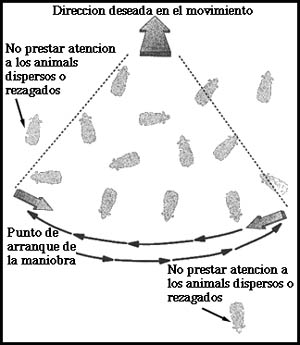
\includegraphics[scale=0.6]{figura111}\\
\centering
\caption{Técnica limpiaparabrisas}
\label{fig:figura111}
\end{figure}


\begin{figure}
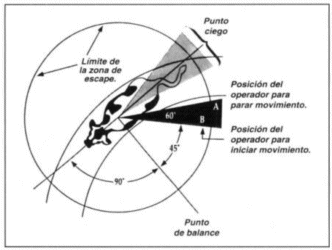
\includegraphics[scale=0.8]{figura112}\\
\centering
\caption{Zona de fuga}
\label{fig:figura112}
\end{figure}


\begin{figure}
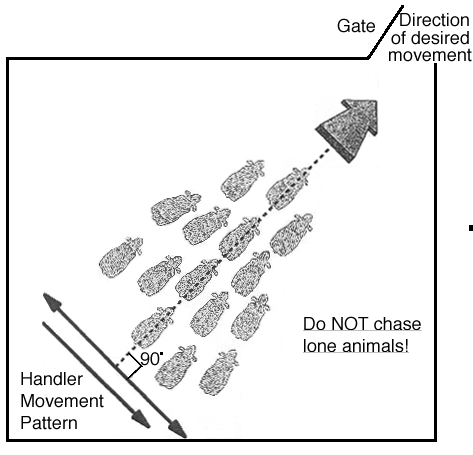
\includegraphics[scale=0.5]{figura113}\\
\centering
\caption{Sacar al ganado: Un controlador}
\label{fig:figura113}
\end{figure}


\begin{figure}
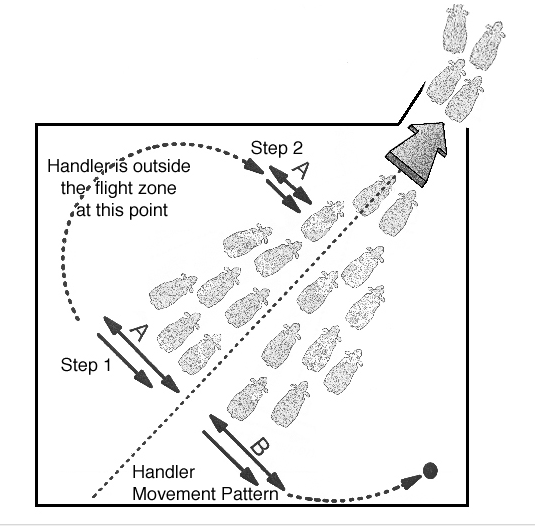
\includegraphics[scale=0.5]{figura114}\\
\centering
\caption{Sacar al ganado: Dos controladores}
\label{fig:figura114}
\end{figure}


\begin{figure}
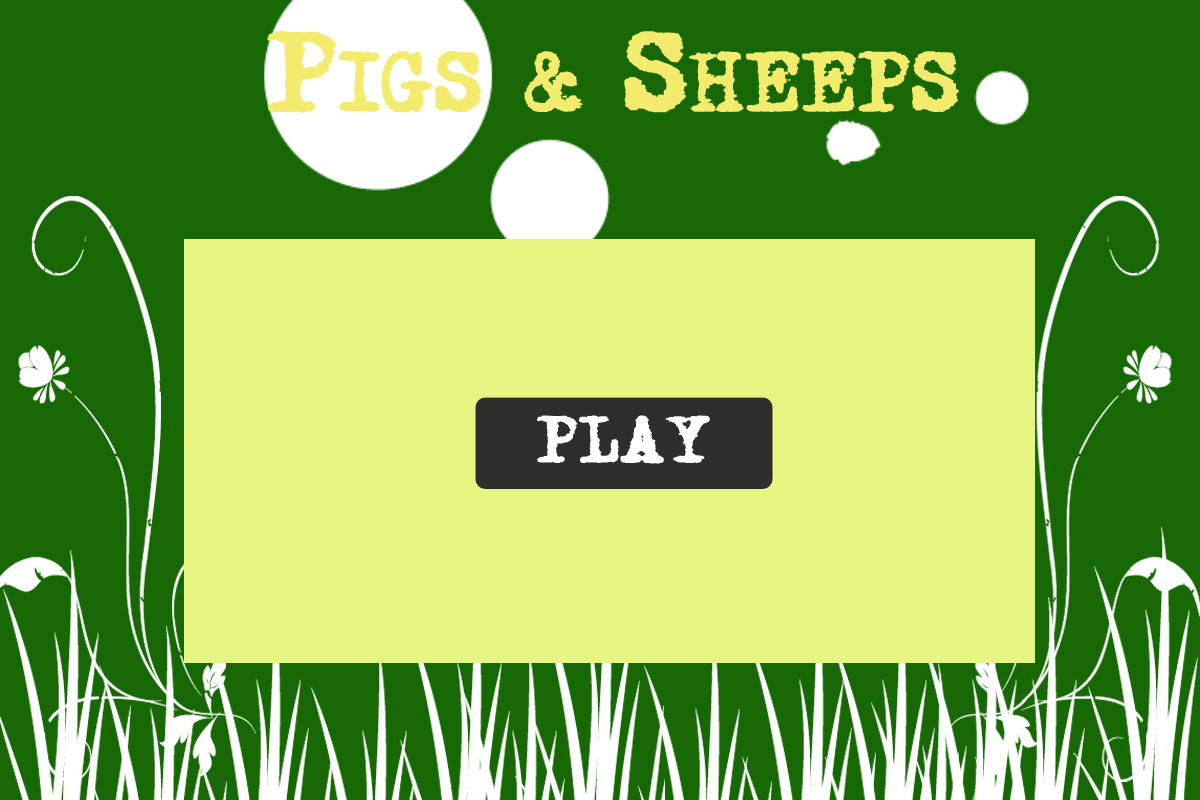
\includegraphics[scale=0.32]{figura311}\\
\centering
\caption{Primer diseño}
\label{fig:figura311}
\end{figure}


\begin{figure}
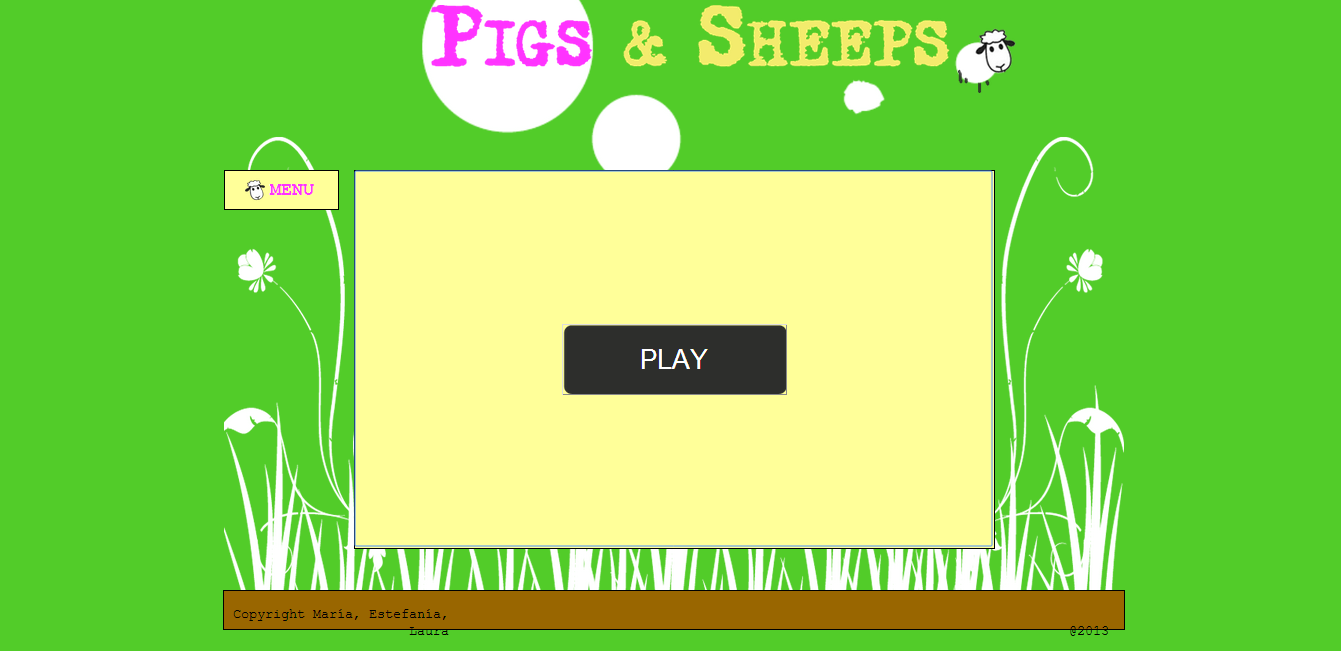
\includegraphics[scale=0.33]{figura312}\\
\centering
\caption{Segundo diseño}
\label{fig:figura312}
\end{figure}


\begin{figure}
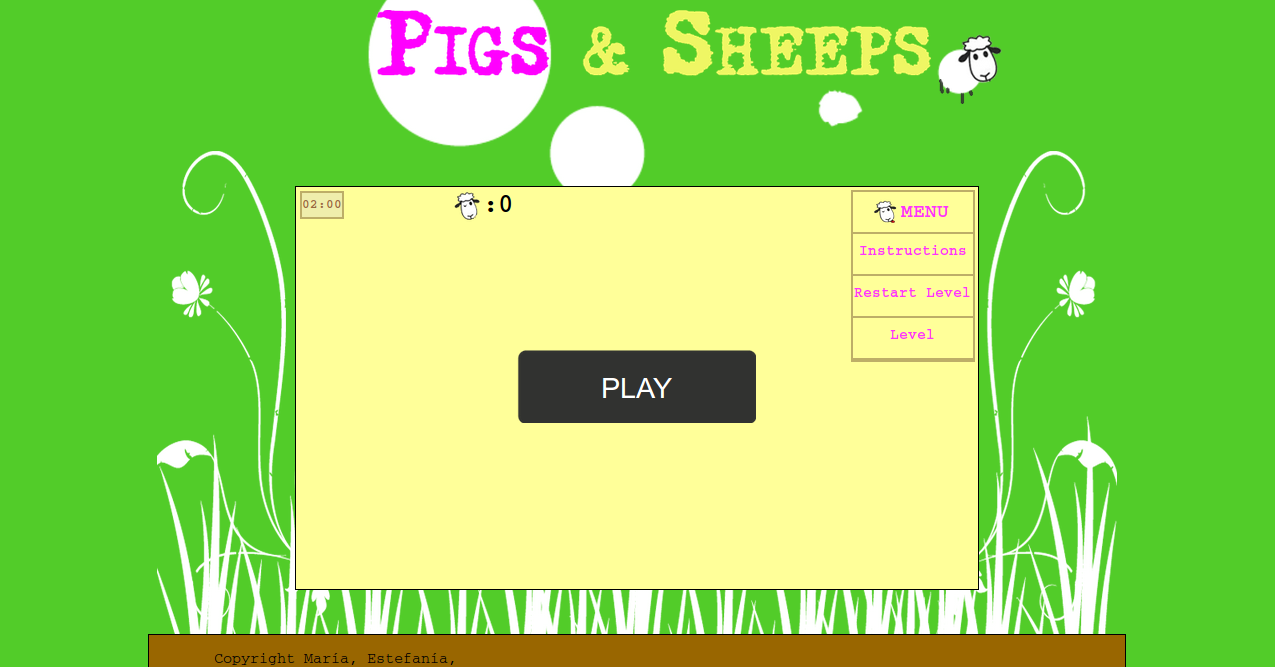
\includegraphics[scale=0.33]{figura313}\\
\centering
\caption{Diseño final}
\label{fig:figura313}
\end{figure}


\begin{figure}
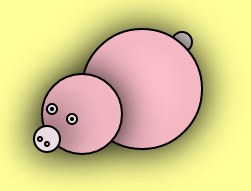
\includegraphics{figura321}\\
\centering
\caption{Primer cerdito}
\label{fig:figura321}
\end{figure}


\begin{figure}

\includegraphics{figura322}\\
\centering
\caption{Oveja - sólo cabeza}
\label{fig:figura322}
\end{figure}


\begin{figure}

\includegraphics{figura323}\\
\centering
\caption{Cerdito definitivo}
\label{fig:figura323}
\end{figure}


\begin{figure}
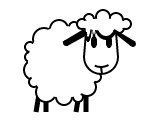
\includegraphics{figura324}\\
\centering
\caption{Oveja definitiva}
\label{fig:figura324}
\end{figure}


\begin{figure}
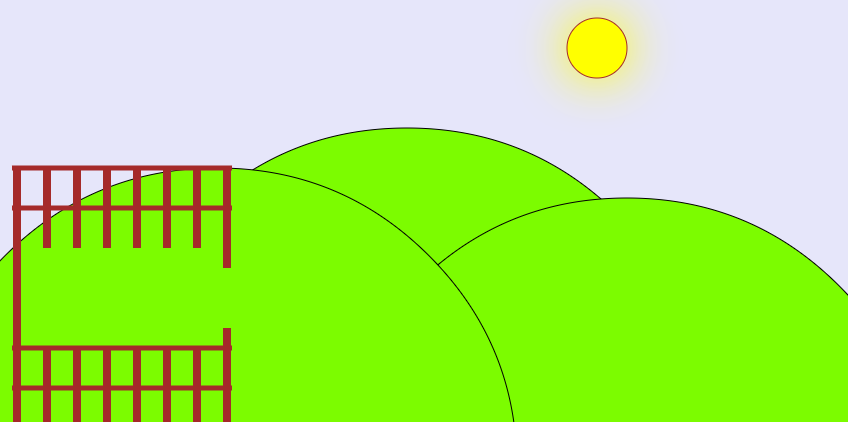
\includegraphics[scale=0.5]{figura325}
\centering
\caption{Primer canvas}
\label{fig:figura325}
\end{figure}


\begin{figure}
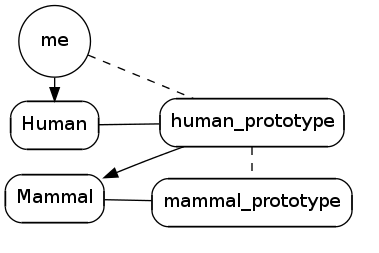
\includegraphics[scale=0.7]{figura413}\\
\centering
\caption{Herencia prototípica}
\label{fig:figura413}
\end{figure}


\begin{figure}
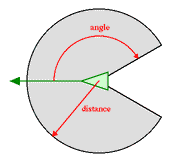
\includegraphics[scale=0.9]{figura4212}\\
\centering
\caption{Radio de un Boid}
\label{fig:figura4212}
\end{figure}

\begin{figure}
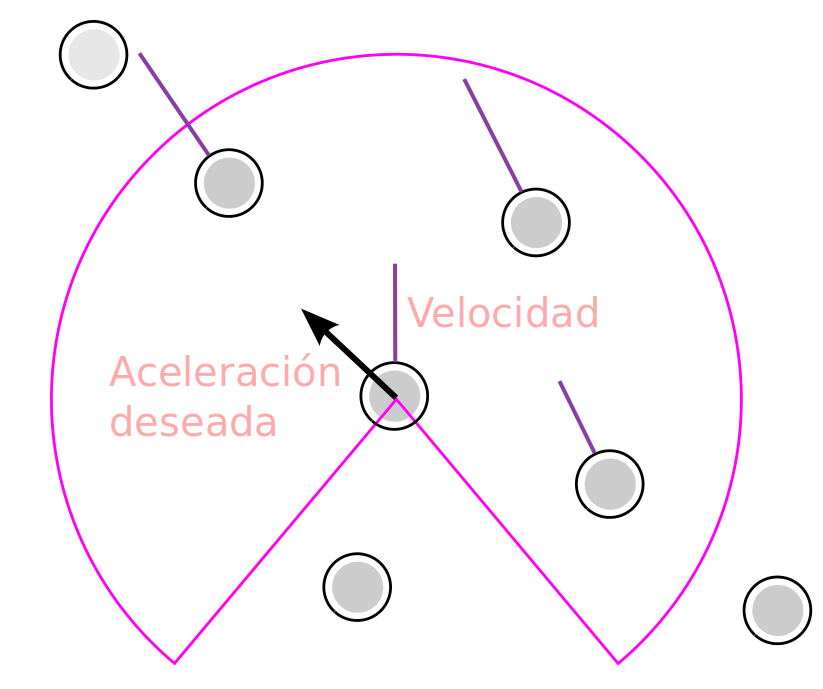
\includegraphics[scale=0.35]{figura4331}\\
\centering
\caption{gráfico de velocidades y aceleraciones}
\label{fig:lock}
\end{figure}
 


\begin{figure}
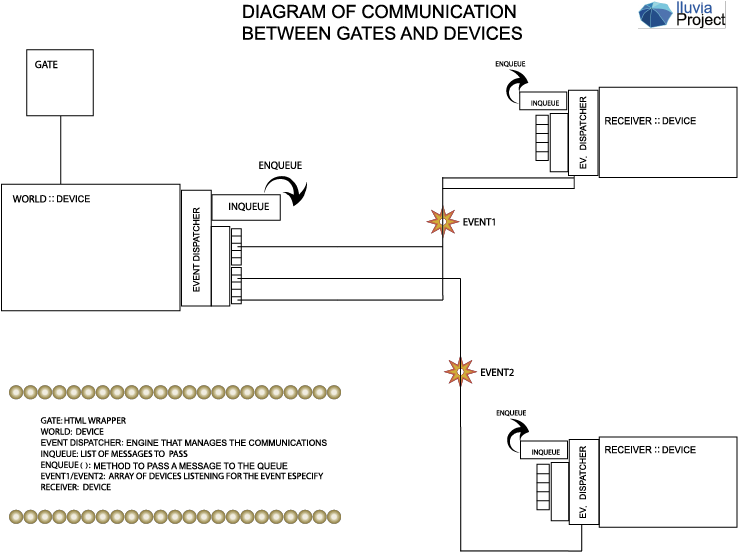
\includegraphics[scale=0.6]{figura511}\\
\centering
\caption{Diagrama Gate y Device}
\label{fig:figura511}
\end{figure}



\section{Cuadros}
\label{sec:cuadros}

\begin{table}[h]
\caption{Comportamientos. Cuadro 4.3.2.1}
% title of Table
%\centering
% used for centering table
\begin{tabular}{| p{4cm} | p{7cm} | p{4cm} |} % centered columns (4 columns)

\hline\hline %inserts double horizontal lines
Nombre de la técnica & Boid cerdito & Boid oveja \\ [0.5ex] % inserts table
%heading
\hline % inserts single horizontal line
% inserting body of the table
Técnica del limpiaparabrisas & El pastor debe moverse en zig-zag detrás de la manada, para mantenerlos en línea recta. & Las ovejas deben de agruparse y moverse en línea recta.\\
Zona de fuga & El cerdito se encuentra en la zona de fuga de la oveja. & La oveja se agita y se enfrenta a él. \\
Moverlos en una manga & El cerdo debe de situarse enfrente del punto de equilibrio & Las ovejas avanzan hacia atrás. \\
Sacar a las ovejas del corral con un controlador & El cerdo se sitúa  a 90º detrás del ganado. Los movimientos deben de ser perpendiculares a los del ganado, hacia delante y hacia atrás sobre la barra transversal de una gigante T. & las ovejas salen en 
manada del corral. \\ [1ex] % [1ex] adds vertical space
\hline %inserts single line
\end{tabular}
\label{table:nonlin} % is used to refer this table in the text
\end{table}
\section{Código}
\label{sec:codigo}

\begin{lstlisting}[caption=Ejemplo de archivo dependencies, label={lst:code211}]
$K\_app\_dependencies = [
    {   module: "Boids", 
        description: "Boids Demo App.",
        path: "",
        files: [
          { name: "brain/behavior\_modifier.js",  
            description: "Self protection behaviors." },
          { name: "brain/behavior.js",           
            description: "Abstract Behavior." },
          { name: "brain/security_behavior.js",  
            description: "Self protection behaviors." },
          { name: "brain/itinerant_behavior.js", 
            description: "Definition of itinerant behaviors."},
          { name: "brain/behavior_group.js",     
            description: "Group of related behaviors."},
          { name: "brain/brain.js",              
            description: "Boid Brain." },
          { name: "boid.js",                     
            description: "One Boid." },
          { name: "world_interface.js",          
            description: "World Interface." },
          { name: "boid_editor.js",              
            description: "Boid panel editor." },
          { name: "world.js",                    
            description: "The world where all boids live."},
          { name: "main.js",                     
            description: "main function." },
        ]
    }
]
\end{lstlisting}

\begin{lstlisting}[caption=Ejemplo clase, label={lst:code411}]
 function Vehicle(mass, number_of_wheels){
  this.mass = mass // In kg 
  this.number_of_wheels = number_of_wheels
  Vehicle.prototype.yield(this)
}

boeing = new Vehicle(20000, 8, 
  function(newly_created_airplane){
    newly_created_airplane.wings = 2
})
\end{lstlisting}


\begin{lstlisting}[caption=Ejemplo clase con funciones, label={lst:code412}]
 var animal = function(limbs, name){
  if (limbs<5)
      return function Mammal(main_food){
          this.name  = name
          this.limbs = limbs
          this.main_food = main_food
      }
    else
      return function Spider(number_of_teeth){
          this.name  = name
          this.limbs = limbs
          this.number_of_teeth = number_of_teeth
      }
}

dog = new (Animal("Tim", 4))("meat")

\end{lstlisting}


\begin{lstlisting}[caption=Objeto configurable Boids, label={lst:code4211}]
 var default_config = {
           geo_data: {
               position: new Vector(Math.floor(Math.random()
                                      * 400), 
                                    Math.floor(Math.random()
                                      * 400)),
               velocity: new Vector(Math.floor(Math.random()
                                      * 40),
                                    Math.floor(Math.random()
                                      * 40)),
               acceleration: new Vector(0,0)
           },
           colour: "blue",

           brain: new Brain(that),
           vel_max: 50,
           mass: 2,
           vision: {radius: 100, angle: 130 * Math.PI / 180},

           force_limits: {
               thrust: 20,
               steering: 50,
               braking: 70
           }
}
\end{lstlisting}

\begin{lstlisting}[caption=Funcion sheep\_limits, label={lst:code4231}]
 Sheep.prototype.sheep\_limits = function() {
    var x\_axis = this.geo\_data.position.Coord[0]
    var y\_axis = this.geo\_data.position.Coord[1]

    if(y_axis >= 800 && x_axis >= 170 || 
       y_axis >= 800 && x_axis <= 274){
           if(this.first_time == 0){
                 this.my_world.max_score = true
                 return
           }
           else
                 return
    }
    if(x_axis <= -445 || x_axis >= 395)
           this.geo_data.velocity.Coord[0] = 0
    if (y_axis >= 800 || y_axis <= 0) {
            this.geo_data.velocity.Coord[1] = 0
    }
}
\end{lstlisting}

\begin{lstlisting}[caption=Funcion update\_physics, label={lst:code4232}]
 Sheep.prototype.update_physics = function(current_time){
    this.last_time = this.current_time
    this.current_time = current_time
    this.geo_data.acceleration = this.requested_acceleration()
    this.geo_data.velocity = integrate(this.geo_data.velocity,
                  this.geo_data.acceleration, this.delta_t() )
    this.sheep_limits()

    if(this.my_world.max_score == true){
            this.my_world.points++
            this.first_time = 1
            this.my_world.max_score = false
    }
    this.geo_data.position = integrate(this.geo_data.position, 
                    this.geo_data.velocity, this.delta_t() )
}
\end{lstlisting}


\begin{lstlisting}[caption=Función first\_draw, label={lst:code4233}]
 Sheep.prototype.first_draw = function() {
    var canvas = document.createElement('canvas');
    canvas.width = 24;
    canvas.height = 24;

    var ctx = canvas.getContext('2d');
}
\end{lstlisting}


\begin{lstlisting}[caption=Función draw, label={lst:code4234}]
 Sheep.prototype.draw = function(ctx){
    var p = this.geo_data.position
    var v = this.geo_data.velocity
    var a = this.geo_data.acceleration
    var radius = 10
    var scale = 1 - p.get_coord(1) / 3000
    var x = this.geo_data.velocity.get_coord(0)

    ctx.save()
    ctx.scale( scale, scale / 2 )

    if(x < 0) {
       ctx.drawImage(this.image, 
                     p.get_coord(0),
                     p.get_coord(1))
    }
    else
       ctx.drawImage(this.image_left, 
                     p.get_coord(0),
                     p.get_coord(1))

    ctx.restore()
}
\end{lstlisting}


\begin{lstlisting}[caption=Función do\_onclick, label={lst:code4235}]
 MouseCoordinates.prototype.do_onclick = function (ev, el) {
   this.X = ev.pageX - screener.offsetLeft
   this.Y = ev.pageY - screener.offsetTop
   this.device.move_shepherd(this.X, this.Y)
}
\end{lstlisting}

\begin{lstlisting}[caption=Función desired\_velocity, label={lst:code4322}]
SheepBehavior.prototype.desired_velocity = function(){
 var arrival_distance
 try{
    arrival_distance = this.target_at().module()
 }catch(err){
    arrival_distance = 0
 }
 var scale = 1
 if(arrival_distance >= 100){
    scale = 0
 }
 else{
    scale = arrival_distance / 100
 }

 return (new Vector(this.target_at().unit().scale(- scale 
                     * this.me.vel_max)))
}
\end{lstlisting}

\begin{lstlisting}[caption=Función set\_target\_at, label={lst:code4341}]
var behaviour = this.shepherd.brain.get_behavior("seek mouse", null)
var x = screen_x - 425
var y = 500 - screen_y
var scale = 1 - y / 3000

behaviour.set_target_at( x / scale, 2 * y / scale)
% \end{lstlisting}


\begin{lstlisting}[caption=Función move\_shepherd, label={lst:code441}]
World.prototype.move_shepherd = function (screen_x, screen_y){
   if (!this.shepherd)
       return
   var behaviour = this.shepherd.brain.get_behavior(
                                        "seek mouse", null)
   var x = screen_x - 425
   var y = 500 - screen_y
   var scale = 1 - y / 3000

   behaviour.set_target_at( x / scale, 2 * y / scale)
}
\end{lstlisting}


\begin{lstlisting}[caption=Función check\_level, label={lst:code442}]
World.prototype.check_level = function() {
    if(this.level == 1 && this.points == 5){
           this.is_finished = true
           this.currentState.requested = this.state.suspended
           this.clock.pause()
           this.winner_pig()
    }
}
\end{lstlisting}


\begin{lstlisting}[caption=Función running\_steady, label={lst:code443}]
World.prototype.running_steady = function(processors_time){
       this.now = processors_time || new Date()
       this.coord_x = this.mouse_coordinates.get_mouse_X()
       this.coord_y = this.mouse_coordinates.get_mouse_Y()

    score_number.style.float = "right"
    score_number.style.fontSize = "24pt"
    score_number.style.marginTop = "5px"
    score_number.style.fontWeight = "bold"
    score_number.innerHTML = ":" + this.points

    this.check_level()
    if(this.is_finished == false)
       this.draw()
}
\end{lstlisting}


\begin{lstlisting}[caption=Función start\_world, label={lst:code451}]
Galactus.prototype.start_world = function() {
   this.world = new World(this.view)
   this.world.level = 1

   this.handler.addPort("restart_game", this)
   
   this.countdown()
   this.playSound()

   var pig = this.world.new_boid_of(Pig, function(config) {
       config.brain.activate("seek mouse", null)
   })

   this.world.shepherd = pig

   var sheeper = [ ]
   for (var i=0; i<30; i++) {
        sheeper.push( this.world.new_boid_of(Sheep, 
           function(config){
             config.geo_data.position = new Vector(
                 Math.floor(Math.random()*400), 
                 Math.floor(Math.random()*400) )
             config.geo_data.velocity = new Vector(
                 Math.floor(Math.random()*20), 
                 Math.floor(Math.random()*20)  )
             config.geo_data.acceleration = new Vector(0,0)
             config.vel_max = 70
             config.vision = {radius: 100, angle: 80 * 
                                           Math.PI / 80}           
             config.force_limits = {
                   thrust: 50,
                   steering: 50,
                   braking: 100
             }
             config.brain.activate("alignment")
             config.brain.activate("sheep", pig)
      }))
  }
   this.world.start()
}
\end{lstlisting}

\begin{lstlisting}[caption=Clase Button, label={lst:code512}]
     Button.prototype = new Gate
     Button.prototype.constructor = Button

     function Button(element){
        try {
            if (arguments.length)
                Gate.call(this, element)
        } catch (e) {
            if (\$K_debug_level >= \$KC_dl.DEVELOPER)
                alert("No event handlers were found.
                      \nException: " + e.toSource())
        }
     }

     Button.prototype.do_onclick   = function(event, element){
        alert("You have made click.")
     }
\end{lstlisting}


\begin{lstlisting}[caption=Estado out, label={lst:code5211}]
  [function(){
      this.gate.panel.style.height = "" + 250 +"px" 
  }; ],
\end{lstlisting}


\begin{lstlisting}[caption=Estado getting\_out, label={lst:code5212}]
  [function (){
      if( this.menu_height >= 50 && this.menu_height<=205)
         this.menu_height+=5
      this.gate.panel.style.height = "" + this.menu_height 
                                   + "px"
  };],
\end{lstlisting}


\begin{lstlisting}[caption=Estado getting\_in, label={lst:code5213}]
  [function(){
      if( this.menu_height >=55 ){         
          this.menu_height-=5
      this.gate.panel.style.height = "" + this.menu_height 
                                   + "px"
  },],
\end{lstlisting}

\begin{lstlisting}[caption=Instructions\_option Gate, label={lst:code5221}]
that.newGate("instructions_option", Gate, {do_onclick: 
                     function(event, element) {
                        alert("Move the little pig to
                              place sheeps into the barnyard")
        } })
\end{lstlisting}

\begin{lstlisting}[caption=restart\_option, label={lst:code5222}]
 that.newGate("restart_option", Gate, { do_onclick: 
                     function(event, element) {
            this.device.fireEvent(
                      this.device.newMessage("sync", 
                               "restart_game", this)
                      )
        } })
\end{lstlisting}

\begin{lstlisting}[caption=level\_option, label={lst:code5241}]
that.newGate("level_option", Gate, {do_onclick: function(event, element){
            var levels_container= document.getElementById('level_option_container')
            levels_container.style.display='inline'
        } })
\end{lstlisting}



\appendix
%\chapter{Manual de Usuario}
\label{chap:manual_de_usuario}

\section{El Interfaz}
\label{sec:interfaz}


Bla Bla es un software ...
%\include{./capitulos/presentacion}

\listoffigures
\listoftables
\lstlistoflistings
\end{document}
